
\section{Commiting and Pushing Your Maven Project Back to Git}

\begin{figure}[t]
\centering
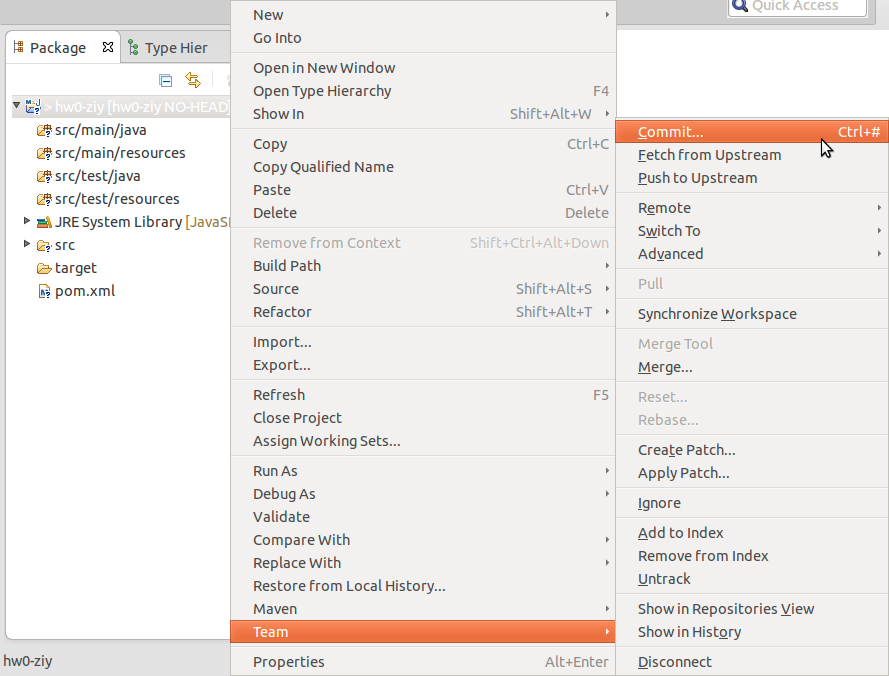
\includegraphics[scale=0.3]{project-19-git-commit}
\caption{Performing a git-commit\label{project-19-git-commit}}
\end{figure}

You should see a ``greater than'' symbol between the project icon and your project name (see Figure \ref{project-19-git-commit}, which means you have made some changes to the project so that there exist some differences between your current workspace version and the branch head. Question marks on the project element icon represent the corresponding elements are not indexed yet. You might be wondering what changes you've made because you thought you haven't written any code. Actually, you have created a Maven project, which process will generate the \verb|pom.xml| file, and modified the Eclipse configuration files. So let's perform our first git-commit.

\begin{enumerate}

\item Right-click on the project name, and select \textbf{Team} $\rightarrow$ \textbf{Commit\ldots}. See Figure \ref{project-19-git-commit}, and then type in your username and email address on GitHub in the popup ``Identify Yourself'' message window.

\begin{figure}[t]
\centering
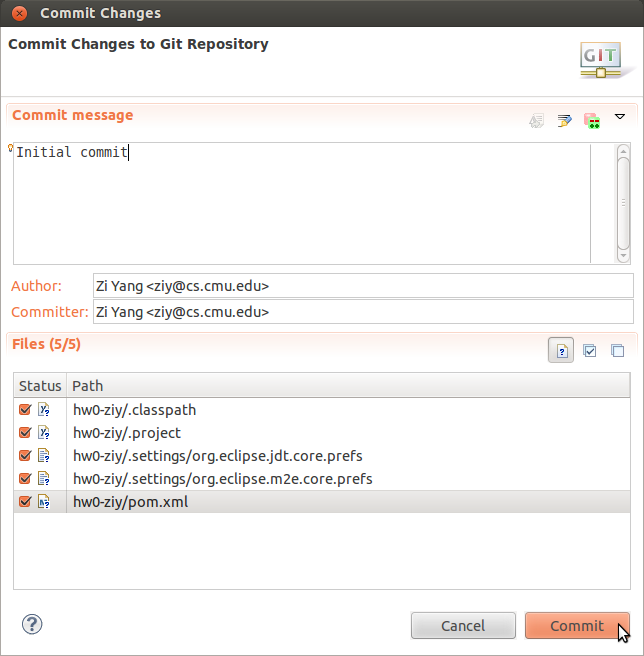
\includegraphics[scale=0.3]{project-21-git-commit-message}
\caption{Viewing and confirming commit message\label{project-21-git-commit-message}}
\end{figure}

\begin{figure}[t]
\centering
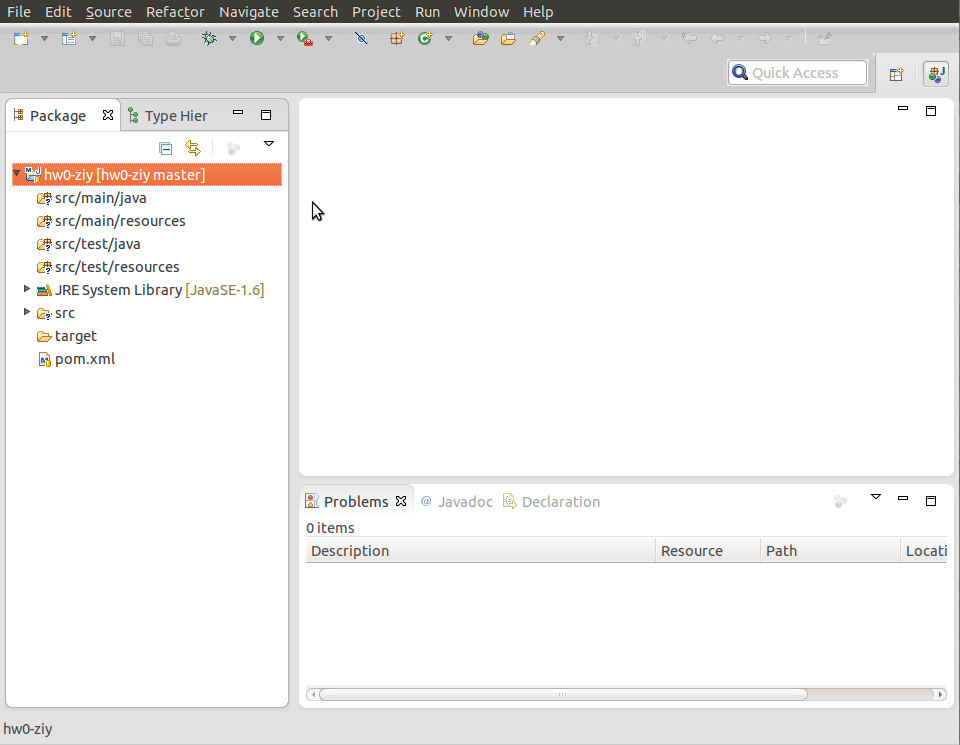
\includegraphics[scale=0.3]{project-22-git-commit-done}
\caption{Committed project\label{project-22-git-commit-done}}
\end{figure}

\item In the ``Commit Changes'' window, you are allowed to choose the files you want to commit (and also automatically add to the index). As you can see in Figure \ref{project-21-git-commit-message}, during creating the empty Maven project, several Eclipse and Maven related configuration files are generated. Moreover, type in a commit message to describe what changes you've made and leave your name as well as your email address (which is a convention) in the committer field. Finally, by clicking \textbf{Commit}, you've done with your first git-commit. You can see in Figure \ref{project-22-git-commit-done}, the ``greater than'' symbol disappears, and the question marks on the committed files become a repository icon, which means the files are in the latest version. You could also find your git-commit helps the code merge into the new master branch from a NO-HEAD branch.

If you are using SVN, then you've done with sychronizing your local workspace with the remote repository once you execute a commit command, but remember the feature of Git? Your project repository is distributed, which means your previous git-commit conceptually affects all your project repositories, but in fact you should make it happen with an additional \emph{push}. A nice picture at \url{http://gitready.com/beginner/2009/01/21/pushing-and-pulling.html} may help you better understand what is actually happening when you perform git commit, add, push, fetch, pull, etc.

\begin{figure}[t]
\centering
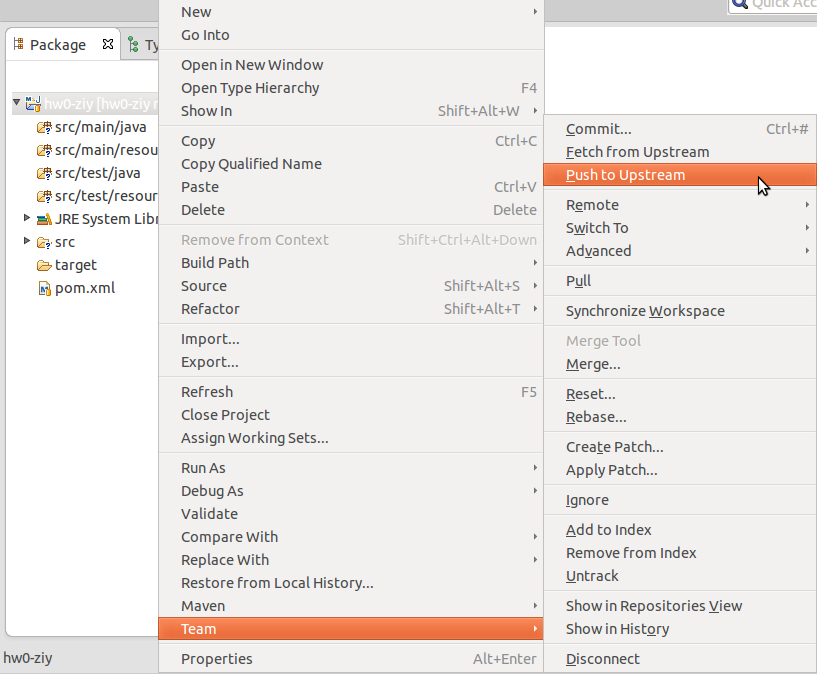
\includegraphics[scale=0.3]{project-23-git-push}
\caption{Performing a git push\label{project-23-git-push}}
\end{figure}

\item Right-click on the project name, and select \textbf{Team} $\rightarrow$ \textbf{Push to Upstream}. See Figure \ref{project-23-git-push}.

\begin{figure}[t]
\hspace{-2em}
\begin{minipage}{0.5\textwidth}
\centering
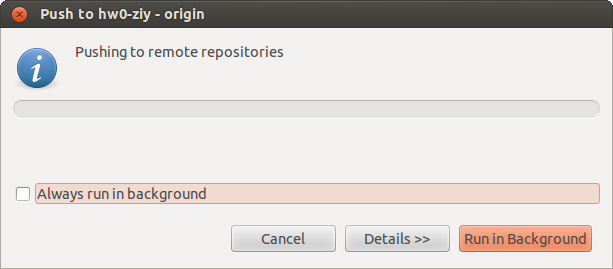
\includegraphics[scale=0.3]{project-24-git-push-progress}
\caption{Viewing the git push progress\label{project-24-git-push-progress}}
\end{minipage}
\hfill
\begin{minipage}{0.5\textwidth}
\centering
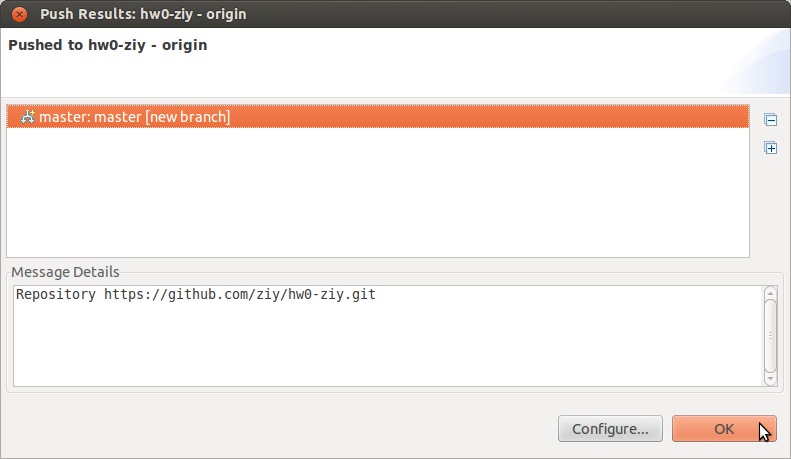
\includegraphics[scale=0.3]{project-25-git-push-result}
\caption{Viewing the git push result\label{project-25-git-push-result}}
\end{minipage}
\hspace{-1em}
\end{figure}

\item Now you can see a progress indication window pops up (see Figure \ref{project-24-git-push-progress}), which says \textbf{Pushing to remote repositories}.
\item Finally, you could see the push results in the ``Push Results'' window. Click \textbf{OK} to close the window and get back to your workspace. 

\end{enumerate}

In your next homework, you will need to use other Git commands within Eclipse.
